\documentclass[tikz,border=0pt]{standalone}
\usepackage[american]{circuitikz}
\usetikzlibrary{arrows.meta,calc,positioning,decorations.pathmorphing,patterns}
\definecolor{zyloTeal}{HTML}{174A5B}
\definecolor{zyloTealTwo}{HTML}{246B7A}
\definecolor{zyloInk}{HTML}{1F2933}
\definecolor{zyloSoft}{HTML}{EAF4F4}
\definecolor{zyloPaper}{HTML}{F8FAFB}
\definecolor{zyloLine}{HTML}{44606B}
\definecolor{zyloOrange}{HTML}{D97706}
\begin{document}
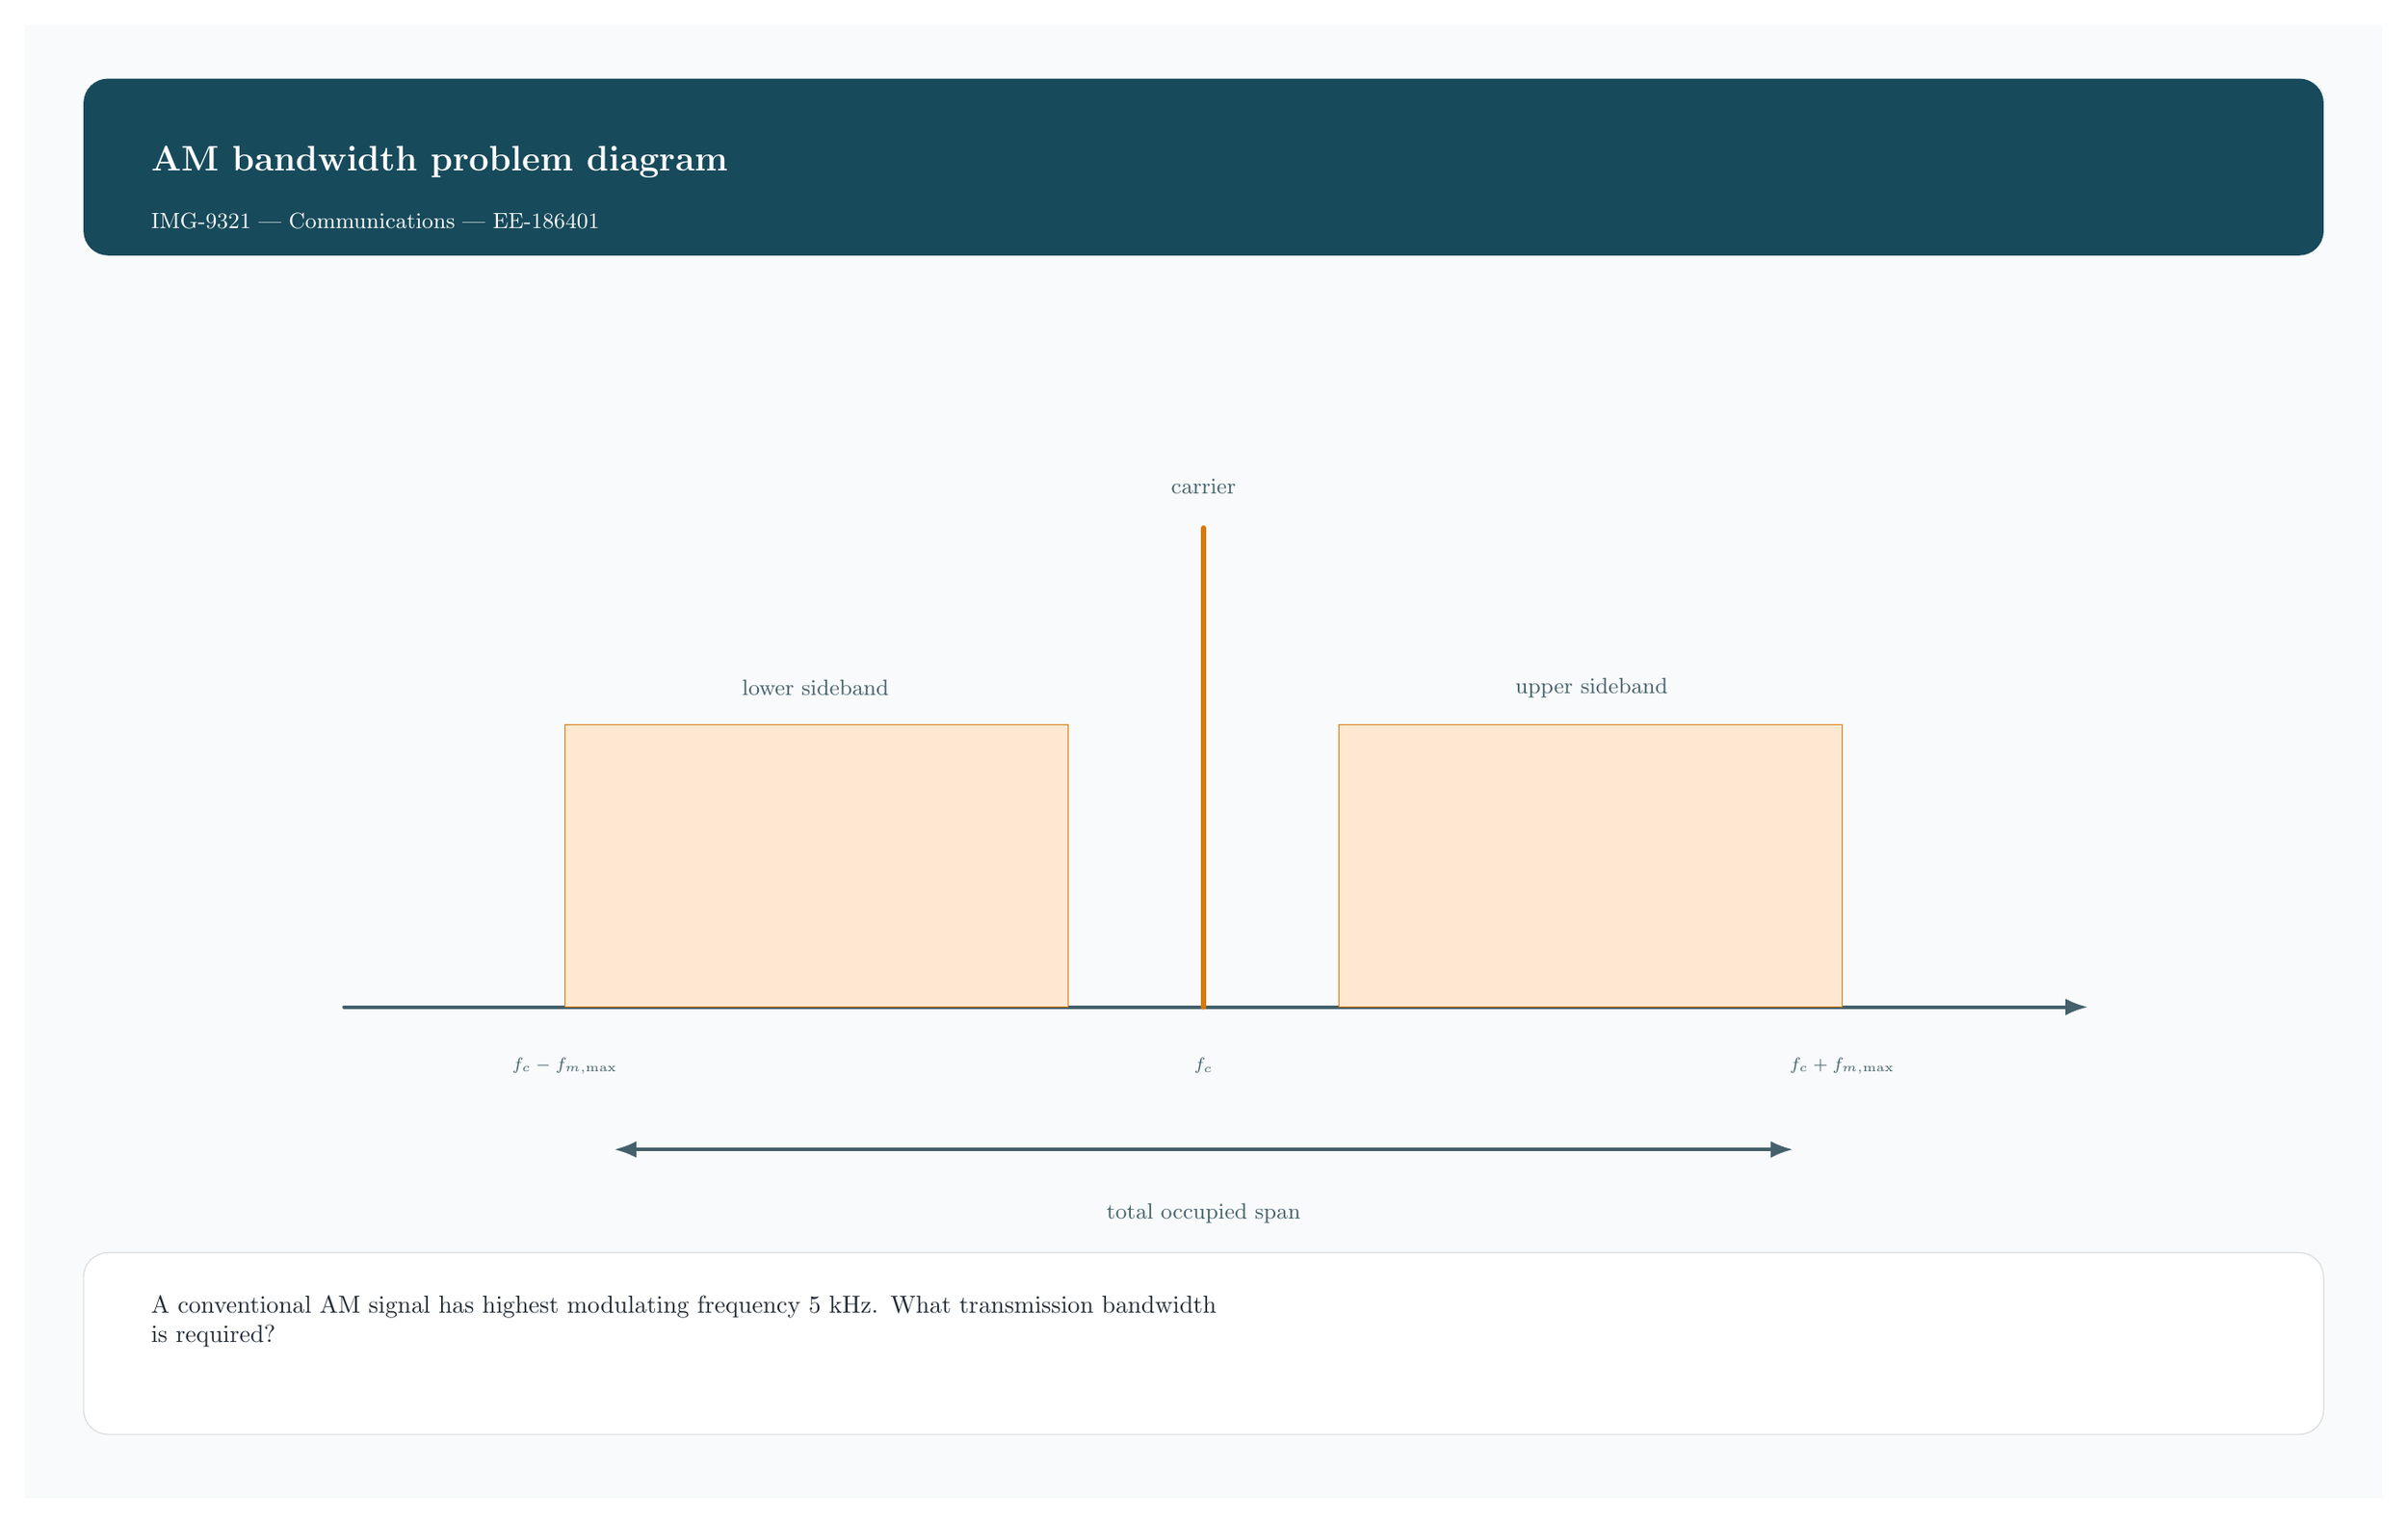
\begin{tikzpicture}[x=1pt,y=-1pt,>=Latex,line cap=round,line join=round]
\path[fill=zyloPaper] (0,0) rectangle (960,600);
\path[fill=zyloTeal,rounded corners=10pt] (24,22) rectangle (936,94);
\node[anchor=west,text=white,font=\bfseries\Large] at (48,56) {AM bandwidth problem diagram};
\node[anchor=west,text=white!82,font=\small] at (48,80) {IMG-9321 | Communications | EE-186401};
\tikzset{wire/.style={draw=zyloTeal,line width=2.2pt},thinwire/.style={draw=zyloLine,line width=1.35pt},accent/.style={draw=zyloOrange,line width=2.2pt},box/.style={draw=zyloTealTwo,fill=zyloSoft,line width=1.5pt,rounded corners=8pt}}
\draw[thinwire,->] (130,400) -- (840,400);
\path[draw=zyloOrange,fill=orange!18] (220,285) rectangle (425,400); \path[draw=zyloOrange,fill=orange!18] (535,285) rectangle (740,400);
\draw[accent] (480,400) -- (480,205);
\node[font=\small,text=zyloLine] at (322,270) {lower sideband}; \node[font=\small,text=zyloLine] at (638,270) {upper sideband}; \node[font=\small,text=zyloLine] at (480,188) {carrier};
\node[font=\scriptsize,text=zyloLine] at (220,424) {$f_c-f_{m,\max}$}; \node[font=\scriptsize,text=zyloLine] at (480,424) {$f_c$}; \node[font=\scriptsize,text=zyloLine] at (740,424) {$f_c+f_{m,\max}$};
\draw[thinwire,<->] (240,458) -- (720,458); \node[font=\small,text=zyloLine] at (480,484) {total occupied span};
\path[draw=black!15,fill=white,rounded corners=10pt] (24,500) rectangle (936,574);
\node[anchor=west,text width=860pt,align=left,text=zyloInk,font=\normalsize] at (48,528) {A conventional AM signal has highest modulating frequency 5 kHz. What transmission bandwidth\\is required?};
\end{tikzpicture}
\end{document}
